\section{Experimental Results}\label{sec:exp}

summary of section\\

\mypar{Experimental setup} All benchmarks and tests were conducted on an Intel
i7-8650U processor with \textit{Intel Turbo Boost} disabled and running at 1.9
GHz. The CPU has a 4$\times$32 KB 8-way associative L1 cache, a 4$\times$256 KB
4-way associative L2 cache and 4$\times$2 MB 16-way associative L3 cache
\cite{intel-opt-manual}.

We chose to benchmark our algorithm with a challenging image depicting a lion
with its cub (\cite{lions}). While some parts of the image, for example the
background, are not quite as hard, their faces to contain a lot of little lines,
dots and other details. As a result, relatively small range blocks are needed to
achieve a reasonable output. Figure \ref{fig:lions} shows the output of the
vectorized code with all four rotations and with error threshold 100 and 3
decompression iterations. For the benchmarks, an error threshold of 300 was used
which means that the quality of the compression is slightly worse but the
running time is shorter.

\begin{figure}[H]
  \centering
  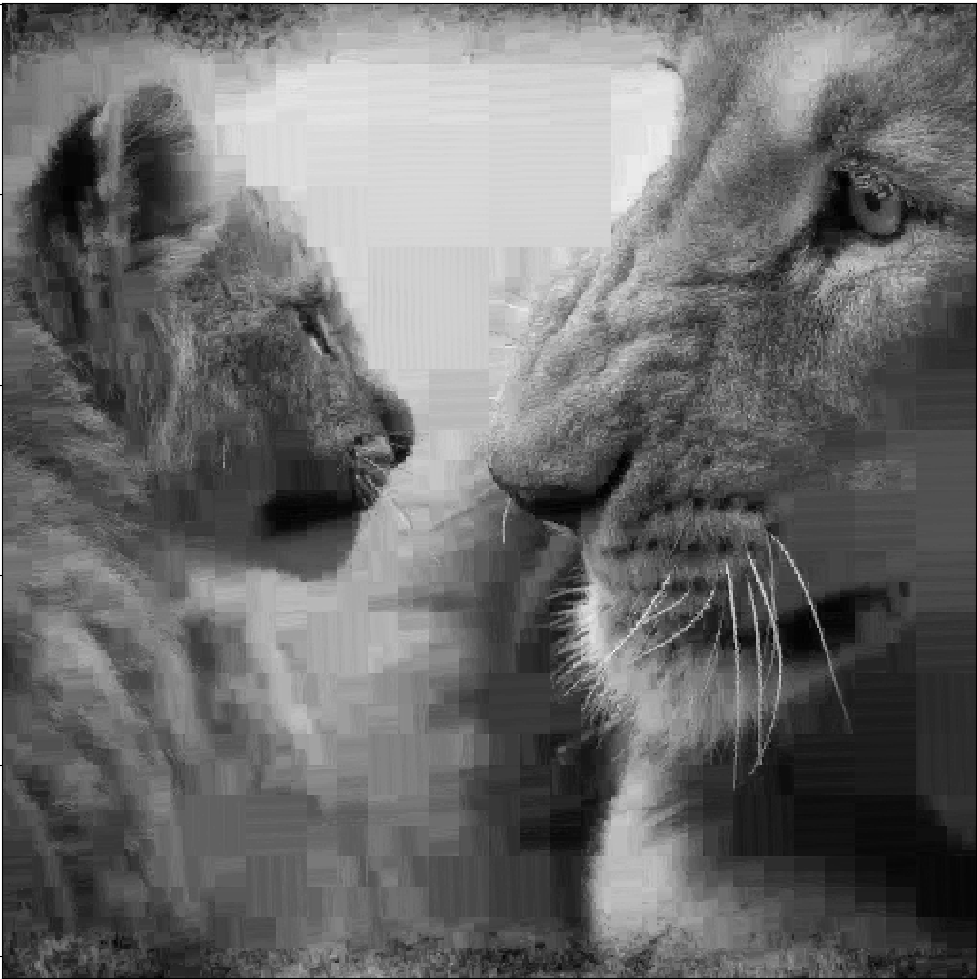
\includegraphics[page=1, width=.45\textwidth]{lion_512_51_e100}
  \caption{Decompressed Image}
  \label{fig:lions}
\end{figure}

\notepascal{should we talk about the PSNR and number of iterations more?}

\mypar{Compiler Flags} Several benchmarks were conducted comparing the achieved
performance using different compiler flags for the \textit{GNU Compiler
  Collection (gcc)} version 9.3.0 and the \textit{Intel C++ Compiler (icc)}
version 19.1.1.217. For all tests \textsc{-march=native} was set.

For both the scalar and the vectorized versions the flag \textsc{-O1} increased
the performance significantly. While \textsc{-O2}, \textsc{-O3} did come with
small improvements for the scalar version (figure \ref{fig:perf_scal}), they did
not make measurable difference for the vectorized version (figure
\ref{fig:perf_vec}). \textsc{-Ofast} was not able increase performance at all
for neither versions.

Intel's compiler was never able to outperform gcc but at least for the
vectorized version it managed to keep up for the larger images (figure\ref{fig:perf_gcc_vs_icc})

\begin{figure}[H]
  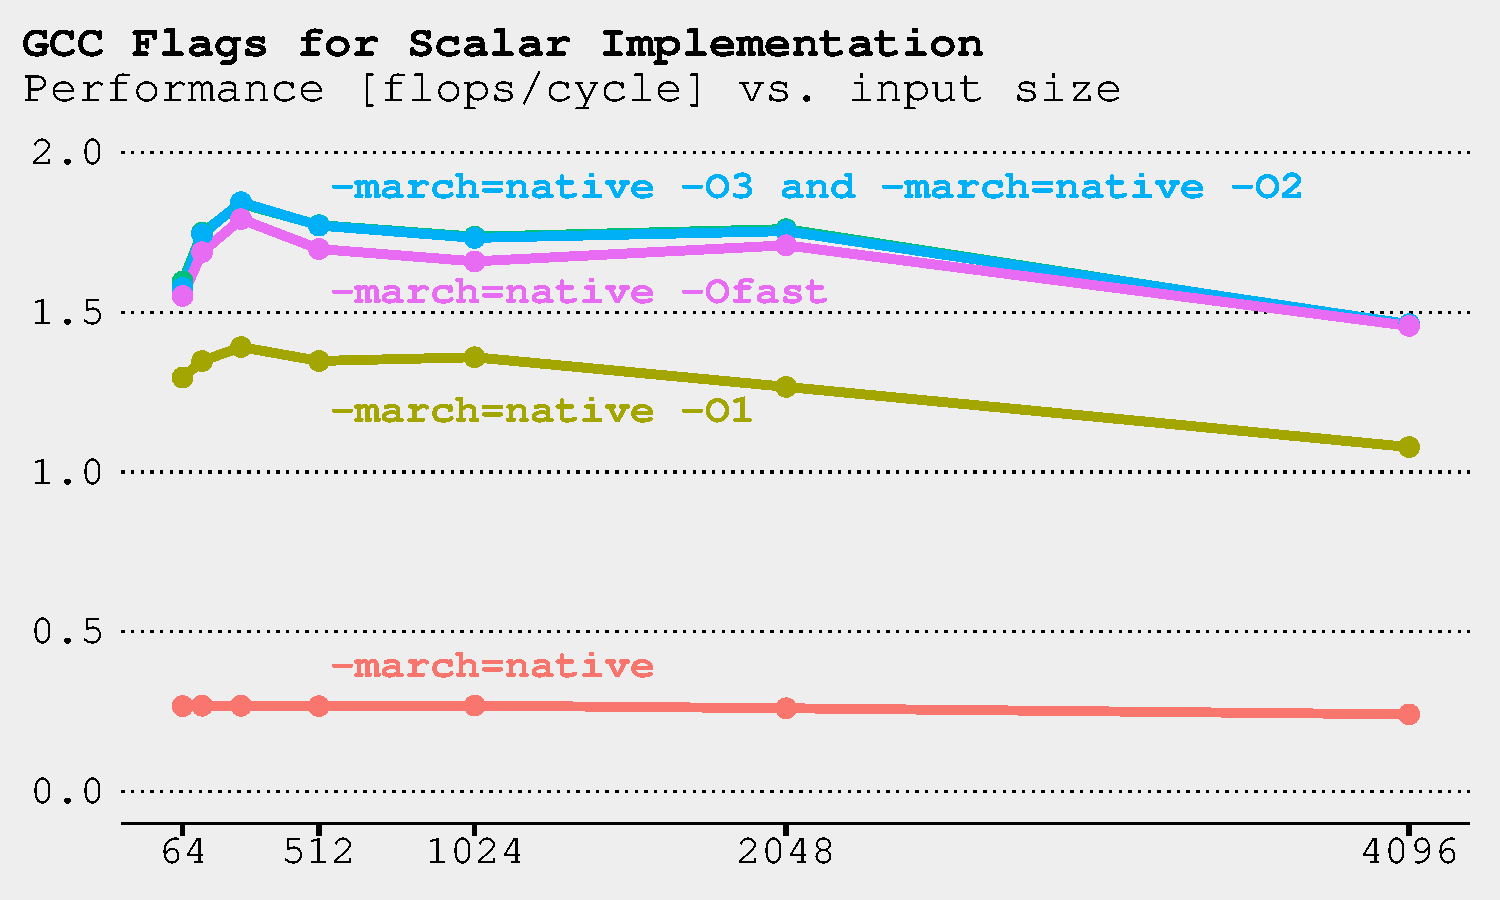
\includegraphics[page=1, width=.45\textwidth]{performance_scalar_opts}
  \caption{Optimization Flags - Scalar Version}
  \label{fig:perf_vec}
\end{figure}

\begin{figure}[H]
  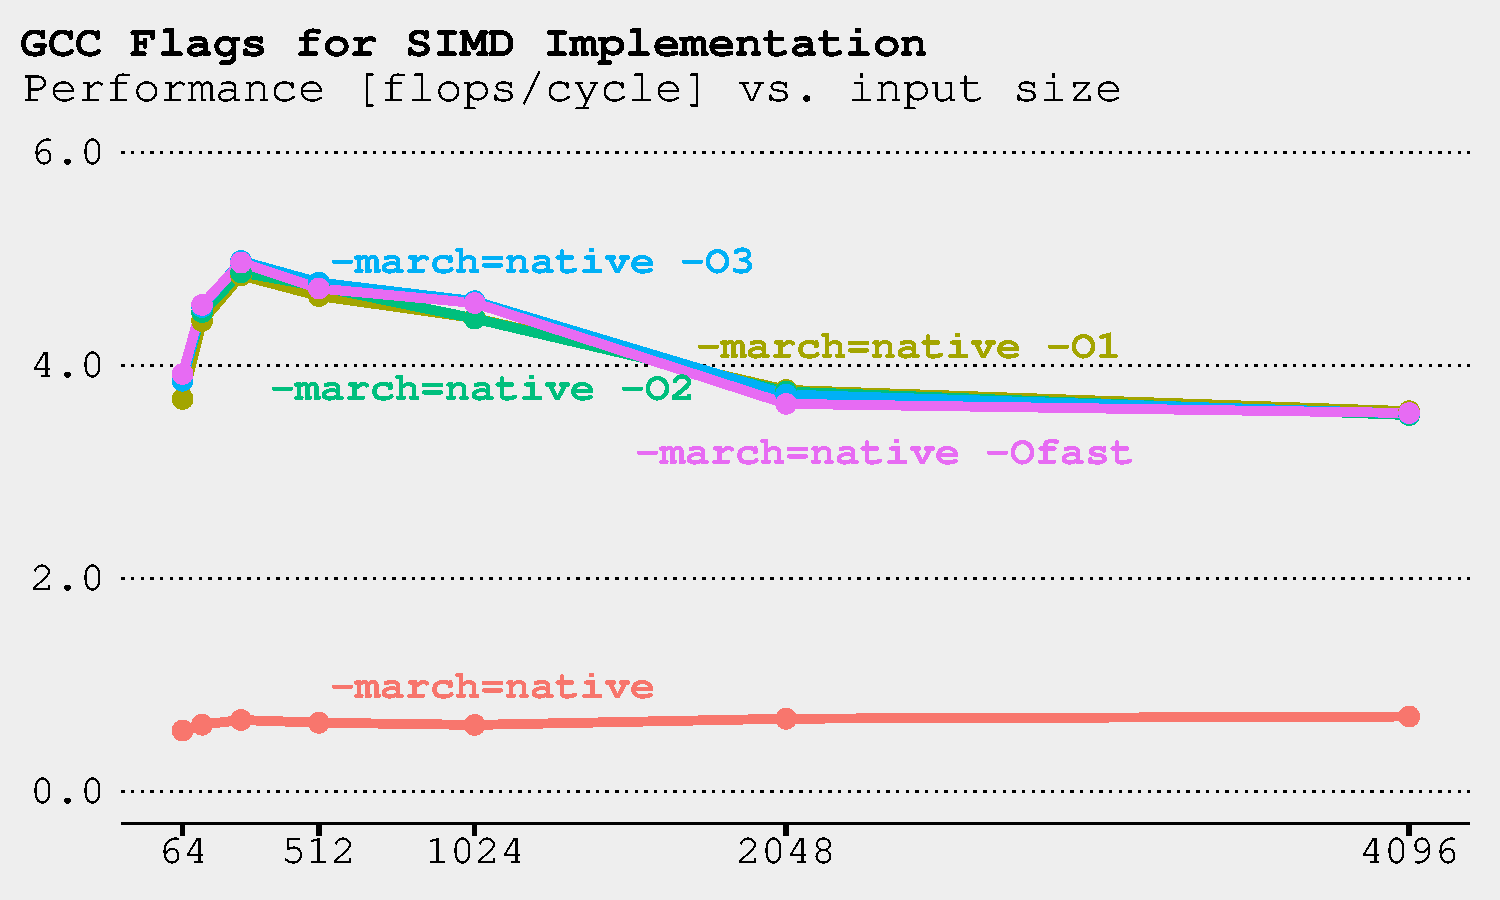
\includegraphics[page=1, width=.45\textwidth]{performance_vectorized_opts}
  \caption{Optimization Flags - Vectorized Version}
  \label{fig:perf_scal}
\end{figure}

\begin{figure}[H]
  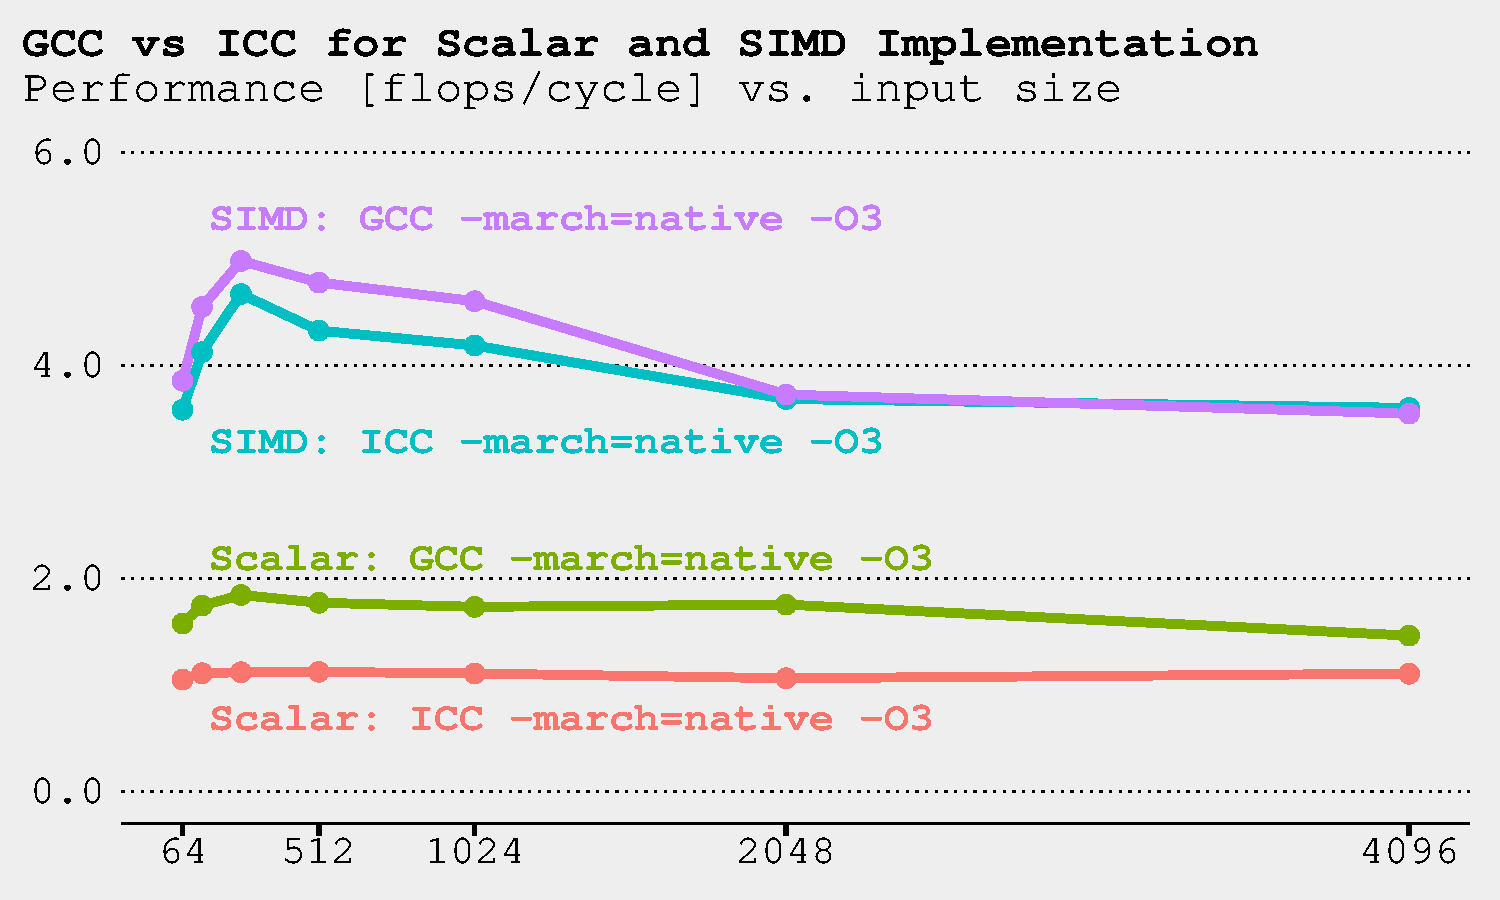
\includegraphics[page=1, width=.45\textwidth]{performance_gcc_vs_icc}
  \caption{GCC vs ICC}
  \label{fig:perf_gcc_vs_icc}
\end{figure}


\mypar{Performance}

\begin{figure}[!ht]
  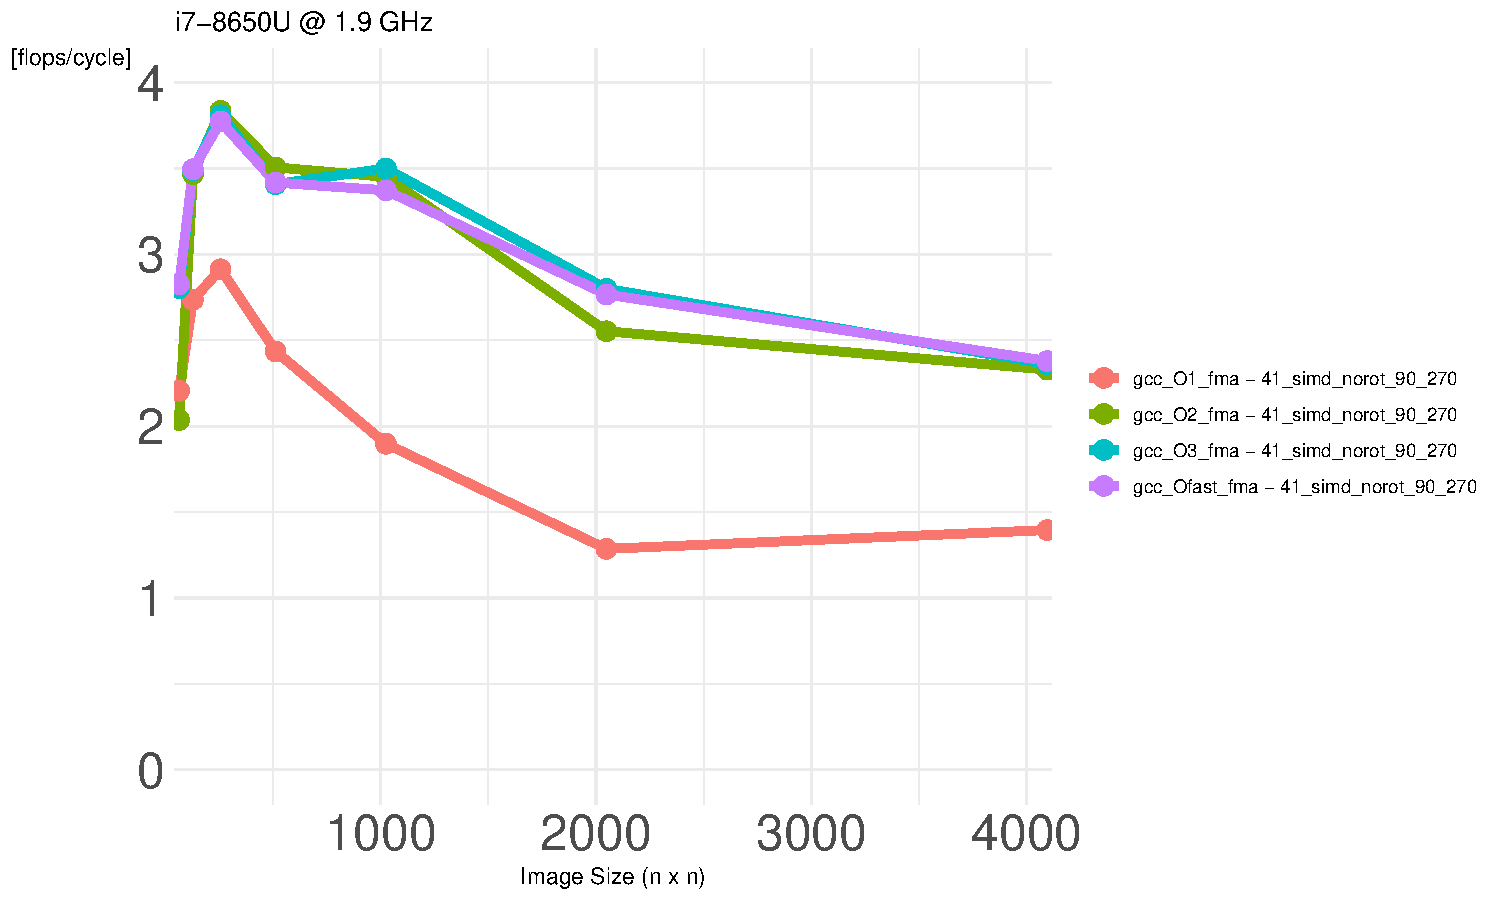
\includegraphics[page=1, width=.45\textwidth]{performance}
  \caption{Performance}
\end{figure}

%%%%%%%%%%%%%%%%%%%%%%%%%%%%%%%%%%%%%%%%%%%%%%%%%%%%%%%%%%%%%%%%%%%%%%%%

% Here you evaluate your work using experiments. You start again with a
% very short summary of the section. The typical structure follows.

% \mypar{Experimental setup} Specify the platform (processor, frequency, cache sizes)
% as well as the compiler, version, and flags used. I strongly recommend that you play with optimization flags and consider also icc for additional potential speedup.

% Then explain what input you used and what range of sizes. The idea is to give enough information so the experiments are reproducible by somebody else on his or her code.

% \mypar{Results}
% Next divide the experiments into classes, one paragraph for each. In the simplest case you have one plot that has the size on the x-axis and the performance on the y-axis. The plot will contain several lines, one for each relevant code version. Discuss the plot and extract the overall performance gain from baseline to best code. Also state the percentage of peak performance for the best code. Note that the peak may change depending on the situation. For example, if you only do additions it would be 12 Gflop/s
% on one core with 3 Ghz and SSE and single precision floating point.

% Do not put two performance lines into the same plot if the operations count changed significantly (that's apples and oranges). In that case first perform the optimizations that reduce op count and report the runtime gain in a plot. Then continue to optimize the best version and show performance plots.

% {\bf You should}
% \begin{itemize}
% \item Follow to a reasonable extent the guide to benchmarking presented in class, in particular
% \item very readable, attractive plots (do 1 column, not 2 column plots
% for this class), proper readable font size. An example is below (of course you can have a different style),
% \item every plot answers a question, which you pose and extract the
% answer from the plot in its discussion
% \end{itemize}
% Every plot should be referenced and discussed (what does it show, which statements do
% you extract).
